\documentclass{article}


% if you need to pass options to natbib, use, e.g.:
%     \PassOptionsToPackage{numbers, compress}{natbib}
% before loading neurips_2022


% ready for submission
\usepackage[final]{neurips_2022}


% to compile a preprint version, e.g., for submission to arXiv, add add the
% [preprint] option:
%     \usepackage[preprint]{neurips_2022}


% to compile a camera-ready version, add the [final] option, e.g.:
%     \usepackage[final]{neurips_2022}


% to avoid loading the natbib package, add option nonatbib:
%    \usepackage[nonatbib]{neurips_2022}


\usepackage[utf8]{inputenc} % allow utf-8 input
\usepackage[T1]{fontenc}    % use 8-bit T1 fonts
\usepackage{hyperref}       % hyperlinks
\usepackage{url}            % simple URL typesetting
\usepackage{booktabs}       % professional-quality tables
\usepackage{amsfonts}       % blackboard math symbols
\usepackage{nicefrac}       % compact symbols for 1/2, etc.
\usepackage{microtype}      % microtypography
\usepackage{xcolor}         % colors
\usepackage{graphicx}


\title{Separation of Research Data from Its Presentation}


% The \author macro works with any number of authors. There are two commands
% used to separate the names and addresses of multiple authors: \And and \AND.
%
% Using \And between authors leaves it to LaTeX to determine where to break the
% lines. Using \AND forces a line break at that point. So, if LaTeX puts 3 of 4
% authors names on the first line, and the last on the second line, try using
% \AND instead of \And before the third author name.


\author{%
https://github.com/t46/separation-data-presentation/graphs/contributors
\thanks{
  LaTeX source is available at 
  \href{https://github.com/t46/separation-data-presentation}.
  }
}


\begin{document}


\maketitle


\begin{abstract}
  This is a position paper proposing the idea of separating research data from its presentation, or view. Today, researchers must not only produce the results of their research but must also think about how to present them. Moreover, in many cases, it is a matter of determining how well the results are displayed within the display format of a single paper. This has caused research results to be unnecessarily difficult to read and research to be unacceptable due to poor presentation. Therefore, we propose to allow separate creators of research data and creators of its display. This can lead to the following benefits: adoption of display formats for different purposes, utilization of buried data, improved reproducibility of studies, and gradual transition to better display formats.
\end{abstract}


\section{Introduction}

\begin{figure}[htb]
    \centering
    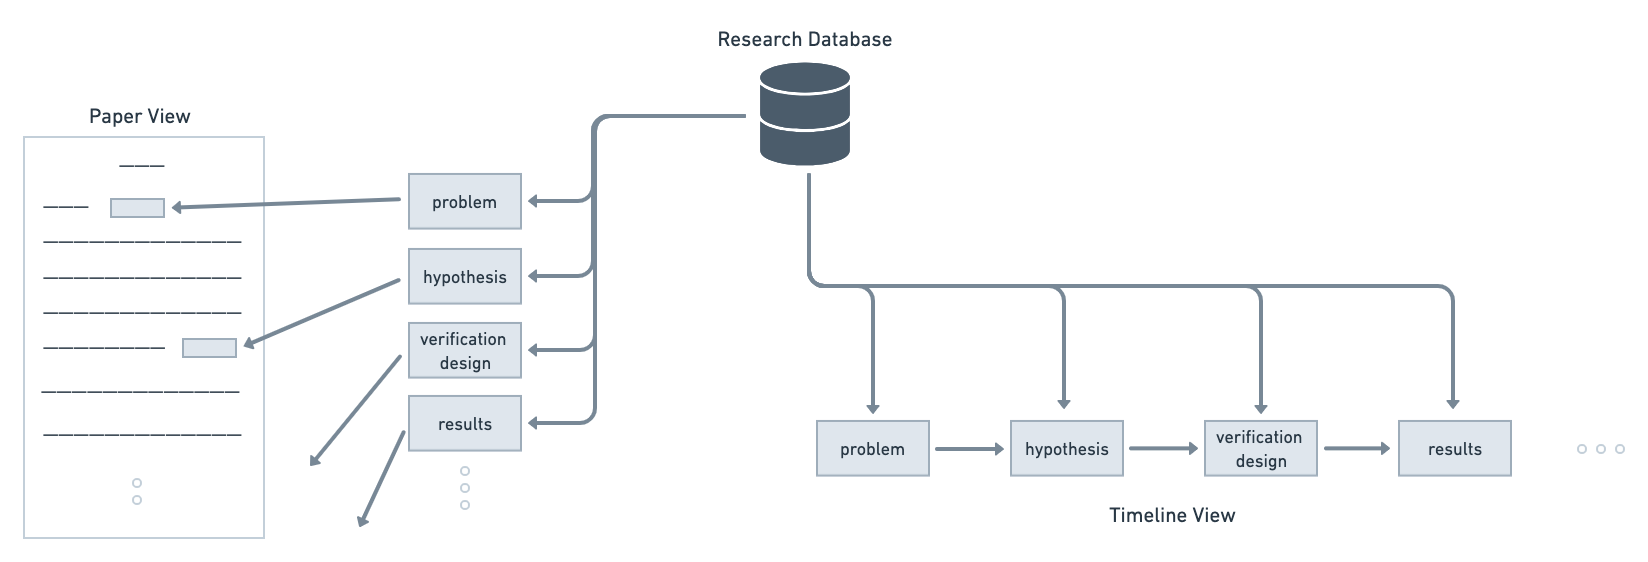
\includegraphics[width=\linewidth]{figs/paper_as_a_view.png}
    \caption{Diagram of the proposed idea of separating research data from its presentation. You store any intermediate products generated by your research in the research database. People around the world then query data from that database and create different views for their purposes.}
    \label{fig:paper_as_a_view}
\end{figure}

Researchers are usually responsible not only for generating research results but also for what and how they present. Even interesting or important research results may not be published if they are not relevant to the claims of the paper. Or, it is often the case that a paper is rejected just because it is poorly written, while the research results are interesting. This means that scientific findings that might have been publicized are no longer publicized just because of the way it is displayed. This is a great loss to human knowledge accumulation.

Another issue researchers face is that they are required to present their findings in a single display format: a research paper. The research paper is an optimal format in an era when printing was the norm. Given today’s advances in information technology, this is not probably optimal today as well. Also, what kind of information you want from a paper depends on who reads it, when reading it, what background they have, etc. More specifically, what readers want to get from a research paper will vary depending on whether they read it during a survey or an experimental design, for example. Furthermore, the optimal format for displaying results will probably differ between research areas such as literature and physics. However, we currently express all of them as a research paper. In other words, we force a single display format to meet several different demands. This makes it unnecessarily difficult to gain insight from research results. This might have slowed the development of science.

The above problems are happening because the research results and their display have become closely intertwined. To solve this problem, we propose to separate research data from its presentation (we call the presentation \textit{view}). We then propose to make it possible to separate the contributors who produce the research results (the researchers as before) from the contributors who produce the format in which they are displayed. Specifically, we will discuss the effectiveness of making research results, including intermediate products, available as a database so that researchers around the world can contribute to the creation of its view. In a nutshell, our suggestion is to store the research process in a database so that anyone can manipulate the view for their purposes.

For example, you may be able to reproduce the entire process of the research by arranging the data stored in the database in chronological order (timeline view). Suppose that you conducted multiple experiments that require interpretation across them. Then, it may be a good idea to use a format that allows you to follow the logical structure more intuitively (logical structure view). Allowing the change in the view of the research data according to the purpose would contribute to the utilization of research results that have been buried in the past.


\section{Proposed Idea}
As stated above, we propose to separate research data from its view. First, any intermediate products generated by the study are stored in a database. When you put it in the database, you give it a label with the necessary information for the view you want to run later. For example, if the relationship between the experimental results and the hypothesis is likely to be complex, the data corresponding to the hypothesis should be labeled ``hypothesis'' and the data corresponding to the experimental results should be labeled ``experimental results''. In general, finer granularity labeling will be needed to achieve more meaningful views. The way the database is created is arbitrary, but something like a relational database may be appropriate. Researchers will make the database public once the results of the study are available. Researchers around the world can then retrieve data from the database and display it in a format suitable for their purposes. The views and interpretation results are then linked to the original database in some way.

\section{Advantage of Splitting Research Result Data and Their View}
\subsection{Single responsibility of a view}
The first advantage is that it eliminates the need to request that a single display format perform multiple functions. Let us take a display format, a research paper,  as an example. 

Currently, we ask for a paper to serve several functions as a display format. First, a research paper is a ``report.'' Therefore, it should convey the necessary information to the intended audience efficiently. Second, a research paper is an ``asset'' cited by other studies. So, it must be comprehensive and rigorous enough to reproduce the original results. Finally, a research paper is a de facto “submission” (not desirable, though). To pass the peer review process of top journals, researchers try their best to make their papers look more appealing.

It is not hard to imagine that these requests can conflict. These complicated demands make reading and writing papers unnecessarily difficult. For instance, it can be difficult to understand the limitation of the research from the paper written to appeal to its positive results. Alternatively, some papers are so carefully detailed that it is difficult to follow the main claims.

Having multiple views of a research database allows us to separate these functions in the form of, for example, ``report views'' or ``stock views.'' You also be able to adopt another structured view suited for your purpose. This is like the \textit{single responsibility principle} in computer programming, which claims that ``\textit{A module should be responsible to one, and only one, actor}'' \cite{martin2018clean}.

This will make acquiring information from papers easier. For example, if you are doing a survey and do not yet know the details of the experiment, you can quickly get to the point by looking at the ``report view'' instead of the ``stock view''. Or, a lengthy proof is difficult to follow the logical development, but a view visualizing the relationships among the complements might make it easier to follow the flow of the proof.

Also, this improves the quality of apprentice researchers’ papers since it does not require complicated technical writing techniques. This would contribute to the publication of more studies with interesting experimental results that otherwise have been rejected just because it was written poorly.

\subsection{Other researchers may find overlooked findings}
A second advantage is that more researchers may be able to find what the authors have not been aware of. Currently, other researchers can only see what those that have done the research decide to display. However, the interpretation of experimental results, for example, varies greatly depending on who is looking at the results and how and where they are looking at them.

The separation of views and data creates room for other researchers to intervene in the interpretation of the outputs of the research process. For example, by freely changing the view, readers can check the soundness of each part of the research process. It prevents authors from cherry-picking results or changing visualization methods to manipulate impressions, and thus avoids being overly critical of the interpretation of study results. This will not only increase the credibility of the study results but will also facilitate the interpretation of the results. 

Also, by adopting a view authors did not, another researcher may be able to find implications from what authors dropped as noise. Bringing different interpretations to experimental results has only been done by collaborators and supervisors. By separating the view from the data, the data will be interpreted from different angles and the perspectives of people with different expertise. In other words, by separating view and dataset, a new form of research collaboration can be realized.

\subsection{More researchers might preserve raw research data}
The third benefit is that it might incentivize researchers to preserve raw data. Until now, authors have had to discard information to be shared to format the paper as a research paper. However, if users can manipulate the view, they can cut the content out when reading by changing the display format as explained above. Thus, readers would request that authors put any missing information in the database to display the views they want to use. And of course, the more information that is stored in the database, as close to the raw data as possible, the more likely it is that you will be able to apply the views you want to perform. Therefore, those who create the view will be making requests to the researchers to keep as much information as possible. Researchers may be motivated to respond and preserve data in a form similar to the raw data. This will help to increase the credibility of scientific knowledge, as more data will be left behind, which is important to reproduce the study.

\subsection{Gradual transition from the paper view to a better view}
The fourth advantage is that it helps gradual transition to a new display format. As mentioned above, the research paper display format is not necessarily optimal. Therefore, it would be preferable to adopt a new display format to present research results. However, immediately abandoning the research paper format and adopting a completely different display format would be a disruptive change. This would make it harder for those accustomed to the research paper format to support the new one. Above all, you must change every past research result published in a research paper format to the new one. This does not seem very feasible.

Positioning the display format of the research paper as one of several views allows you to use the research paper format as well. It is only a matter of time for each generation to decide which display format will eventually become dominant. Also, those accustomed to the existing research paper format can join the new display format by simply using it as a supplementary display format. In this sense, I believe adopting multiple display formats simultaneously, including the research paper format, will help the gradual transition to a better display format. I believe this is a feasible option for display format transition.

\section{Discussion}
In this article, we presented the ideas of splitting research data and their view. And we explained that this could bring several benefits: separating functionality for each display format, promoting the utilization of research results, contributing to improving the reproducibility of research results, and allowing for a gradual transition to a more optimal research results display format.

There are several possible ways to do this, but one way to start is to create a research database in Notion \footnote{https://www.notion.so/}. Notion is a note-taking software platform. It allows you to manage the notes you write as elements of a database. Notion itself does not allow you to create your views. However, Notion has been officially providing an API \cite{notionapi}, so you can read the database using the API. Therefore, by writing your code for a nice view, you can realize a view of the research database.

For each to display the views they wish to see, each piece of data must be given an appropriate label in advance. However, how to label is a difficult question. To answer it, you need to understand what research is and what operations you want to perform on the intermediate outputs of your research. Repeated trial and error would matter for optimal labeling since there are many things you can notice only in practice. In the future, as a research community, we should share our knowledge of appropriate labeling as we compile a database of research data and develop better labeling and views.


\bibliographystyle{unsrt}
\bibliography{ref}

%%%%%%%%%%%%%%%%%%%%%%%%%%%%%%%%%%%%%%%%%%%%%%%%%%%%%%%%%%%%

\end{document}